\chapter{Notions de neurophysiologie}

Nous avons décidé de travailler avec des données de magnétoencéphalographie comme mesure de l'activité cérébrale. Dans cette partie, nous allons alors expliquer comment sont générés ces signaux et comment en obtenir une mesure.

\section{De l'activité neuronale aux signaux neurophysiologiques}

Au sein de l'activité cérébrale, les neurones se transmettent des informations à l'aide de signaux électromagnétiques (au niveau des axones et des dendrites) et chimiques (au niveau des synapses). Les neurones corticaux sont regroupés en un réseau dense et constituent le cortex. Leur activation unitaire (c'est-à-dire le potentiel d'action) consiste en une dépolarisation transitoire de la membrane qui se propage le long des axones. Ces potentiels électriques, transmis le long des axones ou des dendrites, sont appelés courants primaires et correspondent à l'activation proprement dite des neurones \cite{5}. Lorsque ce courant se propage dans le milieu conducteur environnant (liquide céphalo-rachidien, crâne, peau, etc.), il devient un courant de volume. Ces deux types de courant s'additionnent dans le cortex et contribuent aux signaux neurophysiologiques. Lorsque les neurones sont orientés de façon aléatoire, les courants ont tendance à s'annuler. Parce qu'elles sont orientées orthogonalement à la surface de la substance blanche (c'est-à-dire à la surface du cortex), les cellules pyramidales, elles, contribuent principalement aux signaux enregistrés en neurophysiologie. Ces différents cas de figure sont illustrés en Figure \ref{fig1.1}.

\begin{figure}[!ht]
    \centering
    \includegraphics[width=12cm]{activation_neurones.png}
    \caption{Activation neuronale. (a) Neurone seul avec représentation de sont potentiel électrique (ligne pointillée) et du champ magnétique induit (flèche bleue). (b) Groupe de neurones orientés dans le même sens, leur activation synchrone crée un champ magnétique résultant. (c) Neurones orientés de manière aléatoire, les champs magnétiques s'annulent. Adapté de \cite{10}}
    \label{fig1.1}
\end{figure}

\vspace{2ex}
Lorsqu'un groupe de cellules neuronales contiguës s'active de manière synchrone, elles donnent naissance à un courant macroscopique. Lorsqu'il est détecté, il est représenté par un dipôle de courant. Comme la surface corticale est pliée, ces dipôles peuvent être orientés radialement ou tangentiellement par rapport à la surface du crâne.

\vspace{2ex}
La loi de Biot-Savard indique que pour un courant circulant le long d'un circuit en ligne droite, il existe un champ magnétique orienté de façon circulaire autour de cette ligne \cite{11}. Sa direction dépend de la direction de la charge électrique et est donnée par ce que l'on appelle la "règle de la main droite". Le pouce de la main droite pointe dans la direction du flux de courant (de la polarité négative à la polarité positive), les autres doigts pliés indiquent le sens du champ magnétique.

\vspace{2ex}
Cette propriété est importante car elle permet aux physiologistes et aux médecins d'explorer sous deux angles différents (avec des potentiels électriques et des champs magnétiques) la même activité cérébrale en recourant à des techniques différentes.

\vspace{2ex}
Cette activité reflète directement le traitement d'un ensemble de neurones spécifiques et peut être enregistrée de manière invasive (SEEG) ou non invasive (EEG, MEG).

\section{La technique d’enregistrement MEG}

L'activité cérébrale peut être mesurée à différentes échelles et à l'aide de différentes grandeurs. Il existe deux grandes familles de mesures de l'activité cérébrale : celles qui capturent les fluctuations hémodynamiques (modulations du flux, du volume sanguin, etc.), comme l'IRMf, et les mesures de l'activation neuronale réelle, comme l'EEG, la MEG et la SEEG (Figure \ref{fig1.2}). Ces dernières sont appelées techniques neurophysiologiques. Elles enregistrent l'activité électromagnétique des neurones, comme décrit dans la section précédente.

\begin{figure}[!ht]
    \centering
    \includegraphics[width=12cm]{techniques_enregistrement.png}
    \caption{Illustration des différentes techniques d'enregistrement du cerveau. À gauche : techniques mesurant l'hémodynamique. À droite : Techniques neurophysiologiques. Adapté de \cite{12}}
    \label{fig1.2}
\end{figure}

\vspace{2ex}
L'EEG et la MEG sont les deux principales techniques d'enregistrement non invasives utilisées pour mesurer l'activité neurophysiologique au niveau du cortex entier. Il s'agit de techniques standards largement utilisées pour l'étude des activités physiologiques ou pathologiques dans les réseaux cérébraux à grande échelle, avec une résolution temporelle de l'ordre de la milliseconde \cite{9}. Elles se distinguent les unes des autres par la nature du signal recueilli. Alors que l'EEG mesure l'activité cérébrale en termes de potentiels électriques, la MEG enregistre les champs magnétiques provenant de l'activité cérébrale.

\vspace{2ex}
Il en va maintenant de se focaliser sur la technique d'enregistrement d'intérêt pour ce stage, à savoir, la MEG. Les paragraphes qui suivent présentent brievement son histoire ainsi que son fonctionnement.

\vspace{2ex}
Les premières mesures MEG ont été réalisées à la fin des années 1960 grâce à la collaboration de deux physiciens nord-américains : David Cohen et James Zimmerman. Initialement utilisés pour mesurer l'activité cardiaque, les premiers systèmes d'enregistrement MEG n'étaient composés que de quelques capteurs ; ce n'est qu'en 1992 que le premier système pour la tête entière a été construit. Aujourd'hui, les systèmes MEG disposent de plusieurs centaines de canaux organisés en forme de casque couvrant l'ensemble de la tête. Les champs magnétiques générés par l'activité cérébrale sont de l'ordre de quelques dizaines de femtoTesla ($10^{-15}$ Telsa jusqu'à des pico Telsa pour certaines activités cérébrales de grande amplitude telles qu'un pic épileptique). Ces champs très faibles peuvent être mesurés à l'aide de détecteurs magnétiques ultrasensibles appelés SQUID (superconducting quantum interference device), basés sur la supraconductivité et la physique quantique \cite{6}. Couplés à des bobines d'induction, ces dispositifs, immergés dans de l'hélium liquide, peuvent capter de très faibles fluctuations du champ magnétique provenant du cerveau comme on peut l'observer schématiquement en Figure \ref{fig1.3}. 

\begin{figure}[!ht]
    \centering
    \includegraphics[width=15cm]{fonctionnement_meg.png}
    \caption{Illustration de la MEG. Schéma d'un système MEG complet et de ses composants (issu de \cite{5}).}
    \label{fig1.3}
\end{figure}

Comme ces champs magnétiques sont très faibles par rapport à tout autre champ magnétique (le champ magnétique terrestre qui est de l'ordre de $10^{-5}$ ou encore celui d'aimants qui peuvent aller jusqu'à quelques Tesla), un système MEG doit être installé dans une pièce à blindage magnétique pour permettre aux appareils de capter les faibles flucuations. Contrairement à l'EEG, il n'existe pas de position standard pour les capteurs (il n'y a qu'une seule taille de casque). Les positions des capteurs doivent être coregistrées en fonction de l'anatomie du sujet/patient. 

J'ai eu la chance de visiter le centre MEG de la Timone à Marseille, on pourra observer en Figure \ref{fig1.4} des photos prises des différents composants de leur système MEG.

\begin{figure}[!ht]
    \centering
    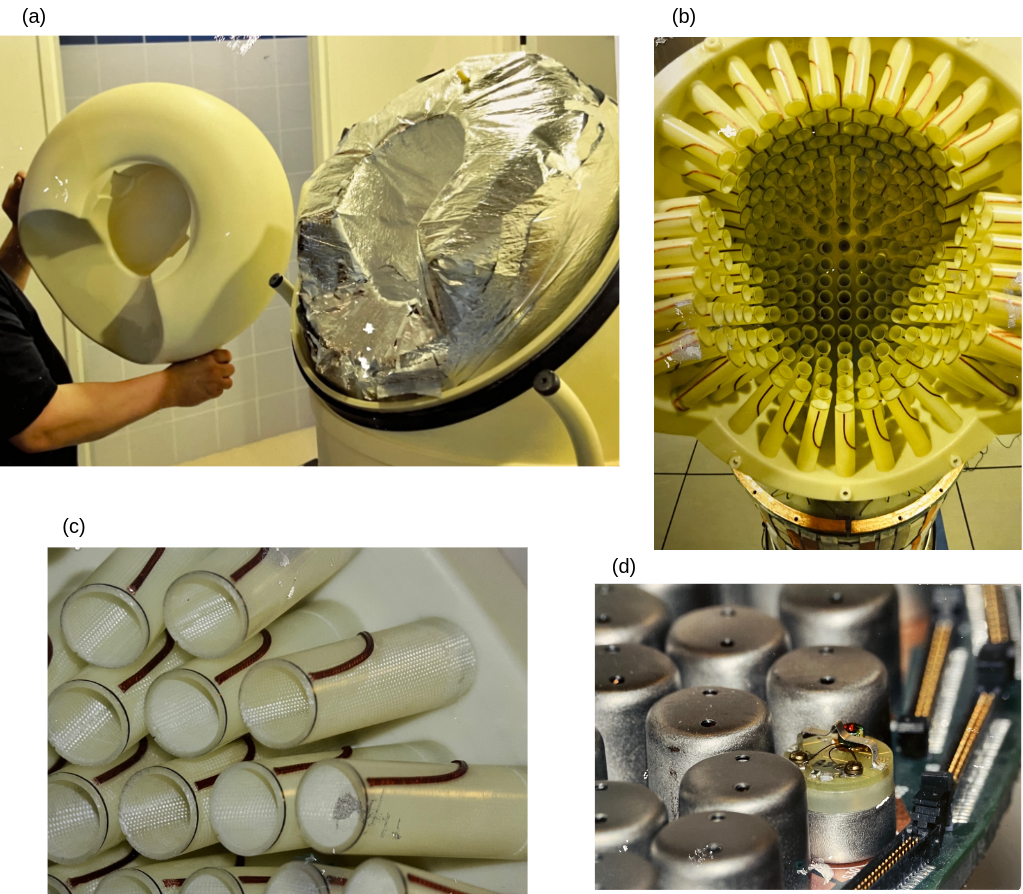
\includegraphics[width=15cm]{illustration_meg.png}
    \caption{Photographies des différents composants du système d'acquisition MEG, prises à différentes profondeurs. (a) Support pour le casque d'acquisition et aperçu de l'isolation du système. (b) Intérieur du dispositif une fois l'isolant retiré où l'on peut apercevoir les SQUID. (c) Gros plan sur les SQUID. (d) Plan correspondant à une prise de vue du dos de la photo précédente, on y voit les bobines.}
    \label{fig1.3}
\end{figure}

